% !TEX root = main-alex.tex


\section{Phase 1: Preprocessing}\label{sec:step1}
% \vspace{-1mm}
\subsection{Small neighborhoods dominators}
% \vspace{-1mm}
As outlined in the introduction, our algorithm works in three phases.
In phase~$i$ for $1\leq i\leq 3$ we select a partial dominating set
$D_i$ and estimate its size in comparison to $D$. In the end we will
return $D_1\cup D_2\cup D_3$. We will call vertices have been selected
into a set $D_i$ \emph{green}, vertices that are dominated by a green
vertex but are not green themselves are called \emph{yellow} and all
vertices that still need to be dominated are called \emph{red}. In the
beginning, all vertices are marked red.

The first phase of our algorithm is similar to the first phase of the
algorithm of Lenzen et al.~\cite{lenzen2013distributed} for planar graphs.
It is a preprocessing step that leaves us with only vertices whose
neighborhoods can be dominated by a few other vertices. Lenzen et al.\
proved that if $G$ is planar, then there exist less than $3\gamma$
many vertices~$v$ such
that the open neighborhood $N(v)$ of $v$ cannot be dominated by $6$
vertices of $V(G)\setminus \{v\}$~\mbox{\cite[Lemma
6.3]{lenzen2013distributed}}. The lemma can be generalized to more
general graphs, see~\cite{amiri2019distributed}. We prove the
following lemma, which is stronger in the sense that the number of
vertices required to dominate the open neighborhoods is smaller than
in~\cite{lenzen2013distributed} and~\cite{amiri2019distributed}, at the cost of having slightly more vertices with that property.



\begin{lemma}\label{lenzen-improved}
  % Let $\nn$ be an integer strictly larger than $\nabla_1^B(G)$, the
  % edge density of a densest bipartite $1$-shallow minor of $G$.
  Let $\hat{D}$ be the set of vertices $v\in V(G)$ whose neighborhood
  cannot be dominated by $(2\nn-1)$ vertices of $D$ other than $v$,
  that is,

  \vspace{-4mm}
  \[
    \text{ $\hat{D}\coloneqq \{v\in V(G) :$ for all sets
      $A\subseteq D\setminus \{v\}$ with $N(v)\subseteq N[A]$ we have
      $|A|> (2\nn-1)\}$.}
  \]


  Then $|\hat{D}\setminus D| < \rho(G)\cdot\gamma$.
\end{lemma}

Remember that $\nn$ is an integer strictly larger than $\nabla_1^B(G)$, the
edge density of a densest bipartite $1$-shallow minor of $G$.
Additionally
$\rho(G)\le\chi(G)\leq 2\nabla_0(G)+1\leq 2\nabla_1+1$. The precise values
will be relevant for the planar case.

\begin{proof}
  Assume $D=\{b_1,\ldots,b_\gamma\}$.  Assume that there are
  $\rho(G)\cdot\gamma$ vertices
  $a_1,\ldots,a_{\rho(G)\cdot\gamma}\not\in D$ satisfying the above
  condition. Be definition of the Hall ratio we
  find an independent subset of the $a_is$ of size~$\gamma$. We can
  hence assume that $a_1,\ldots,a_{\gamma}$ are not connected by an
  edge. We proceed towards a contradiction.

  We construct a bipartite $1$-shallow minor $H$ of $G$ with the
  following \mbox{$2\gamma$} branch sets. For every
  \mbox{$i\le \gamma$} we have a branch set $A_i=\{a_i\}$ and a branch
  set
  $B_i=N[b_i]\setminus \big(\{a_1,\ldots, a_{\gamma}\}\cup
    \bigcup_{j<i}N[b_j]$ $\cup \{b_{i+1},\ldots, b_\gamma\}\big)$. Note that
  the $B_i$ are vertex disjoint and hence we define proper branch
  sets. Intuitively, for each vertex $v\in N(a_i)$ we mark the
  smallest $b_j$ that dominates $v$ as its dominator. We then contract
  the vertices that mark $b_j$ as a dominator together with $b_j$ into
  a single vertex. Note that because the $a_i$ are independent, the
  vertices $a_i$ themselves are not associated to a dominator as no
  $a_j$ lies in $N(a_i)$ for~$i\neq j$.  Denote by
  $a_1',\ldots, a_{\gamma}',b_1',\ldots, b_\gamma'$ the associated
  vertices of $H$. Denote by $A$ the set of the $a_i's$ and by $B$ the
  set of the~$b_j's$.  We delete all edges between vertices of
  $B$. The vertices of $A$ are independent by construction. Hence, $H$
  is a bipartite $1$-shallow minor of $G$.  By the assumption that
  $N(a_i)$ cannot be dominated by $2\nn-1$ elements of $D$, we
  associate at least~$2\nn$ different dominators with the vertices of
  $N(a_i)$. Note that this would not necessarily be true if~$A$ was
  not an independent set, as all $a_j\in N(a_i)$ would not be
  associated a dominator.

  Since $\{b_1,\ldots, b_\gamma\}$ is a dominating set of $G$ and by
  assumption on $N(a_i)$, we have that in $H$, every~$a'_i$ has at
  least $2\nn$ neighbors in $B$. Hence,
  $|E(H)| \ge 2\nn|V(A)| = 2\nn\gamma$. As $|V(H)|=2\gamma$ we
  conclude $|E(H)|\ge \nn|V(H)|$. This however is a contradiction,
  as by assumption~$\nn$ is strictly larger than $\nabla_1^B(G)$ the edge
  density of a densest
  bipartite $1$-shallow minor of $G$.
\end{proof}

% \pagebreak
Let us fix the set $\hat{D}$ for our graph $G$.
\begin{tcolorbox}
\vspace{-4mm}
    \begin{align*}
      \hat D\coloneqq \{v\in V(G) : \text{ for all } A\subseteq D\setminus \{v\}
      & \text{ with $N(v)\subseteq N[A]$} \text{ we have $|A|>(2\nabla-1)\}$.}
  \end{align*}
\end{tcolorbox}
\smallskip
Note that $\hat{D}$ cannot be computed by a local algorithm as we do
not know the set $D$. It will only serve as an auxiliary set in our
analysis.

\smallskip We define $D_1$ as the set of all vertices whose
neighborhood cannot be dominated by $2\nabla-1$ other vertices.
The first phase of the algorithm is to compute the set
$D_1$, which can be done in 2 rounds of communication.

\begin{tcolorbox}[colback=red!5!white,colframe=red!50!black]
  \vspace{-4mm}
  \begin{align*}
  D_1\coloneqq \{v\in V(G) : \text{ for all } A\subseteq V(G)\setminus \{v\}
  & \text{ with $N(v)\subseteq N[A]$ we have $|A|> (2\nabla-1)\}$.}
  \end{align*}
\end{tcolorbox}


\begin{lemma}\label{lem:size-D1}
  $D_1\subseteq \hat{D}$ and hence $|D_1\setminus D|\leq \rho(G)\cdot \gamma$.
\end{lemma}

\begin{proof}
  If the open neighborhood of a vertex $v$ cannot be dominated by $2\nabla-1$
  vertices from $V(G)\setminus\{v\}$, then in particular it cannot be
  dominated by $2\nabla-1$ vertices from $D\setminus\{v\}$.  Hence
  $D_1\subseteq \hat{D}$ and we can bound the size of $D_1$ by that of
  $\hat{D}$.
\end{proof}

\pagebreak
We mark the vertices of $D_1$ that we add to the dominating set in the
first phase of the algorithm as green, the neighbors of $D_1$ as
yellow and leave all other vertices red. Denote the set of red
vertices by~$R$, that is, $R=V(G)\setminus N[D_1]$.  For $v\in V(G)$
let $\Nr(v)\coloneqq N(v)\cap R$ and $\dr(v)\coloneqq |\Nr(v)|$
be the \emph{residual degree} of~$v$, that is, the number of neighbors
of $v$ that still need to be dominated.

\smallskip By definition of $D_1$, the neighborhood of every non-green
vertex can be dominated by at most~$2\nabla$ other vertices. This holds true
in particular for the subset $\Nr(v)$ of neighbors that still need to be
dominated.  Let us fix such a small dominating set for the red
neighborhood of every non-green vertex.

\begin{tcolorbox}
  For every $v\in V(G)\setminus D_1$, we fix
  $A_v\subseteq V(G)\setminus \{v\}$ such that:
    $$N_R(v)\subseteq N[A_v] ~~\text{and}~~ |A_v|\leq 2\nabla.$$

  Additionally, for vertices $v\in V(G)\setminus \hat{D}$, we enforce that
  $A_v\subseteq D\setminus \{v\}$.
\end{tcolorbox}

There are potentially many such sets $A_v$ -- we fix one such set
arbitrarily.
Let us stress that we cannot compute these sets
in a local algorithm as the sets $D$ and $\hat{D}$ are not known
to the algorithm. We only use these sets for our further argumentation.

\subsection{Limitations of the method}

\smallskip
We can apply the above approach to obtain a small set $D_1$ only if $\nabla_1$ is bounded by a constant. For example in graphs of bounded degeneracy in general the number of vertices that dominate the
neighborhood of a vertex can only be bounded by $\gamma(G)$.
Hence, the approach based on covers and pseudo-covers that is employed
in the following cannot be extended to degenerate  graph classes. Below
we show an example where this is the case.


\begin{example}
Let $G(\gamma,m)$ be the graph with vertices $v_i$ for $1\leq i\leq \gamma$,
$w^j$ for $1\leq j\leq m$ and $s_i^j$ for $1\leq i\leq \gamma, 1\leq j\leq m$.
We have the edges $\{v_1, w^j\}$ for $1\leq j\leq m$, hence $v_1$
dominates all~$w^j$. We have the edges $\{w^j, s_i^j\}$ for all $1\leq i\leq \gamma,
1\leq j\leq m$, hence, the $s_i^j$ are neighbors of $w^j$. Finally,
we have the edges $\{v_i, s_i^j\}$, that is, $v_i$ dominates the $i$th
neighbor of $w_j$ (see \cref{fig:example}). Hence, for $m>\gamma$,
$G(\gamma, m)$ has a dominating set of size
$\gamma$ and $m$ vertices whose neighborhood can be dominated
only by~$\gamma(G)$ vertices.
% \cref{lem:neighborhood-dom1} implies
% that $\gamma < 2\nabla_1$, and as we can choose~$m$ arbitrary
% large, we cannot usefully apply \cref{lem:neighborhood-dom1}.
Note that $G(\gamma,m)$ is
\mbox{$2$-degenerate}. As we can choose~$m$ arbitrary
large, we cannot usefully apply the method based on
\cref{lem:size-D1} for degenerate classes in general.

\vspace{-3mm}
\begin{center}
  \begin{figure}[h]
    \center
    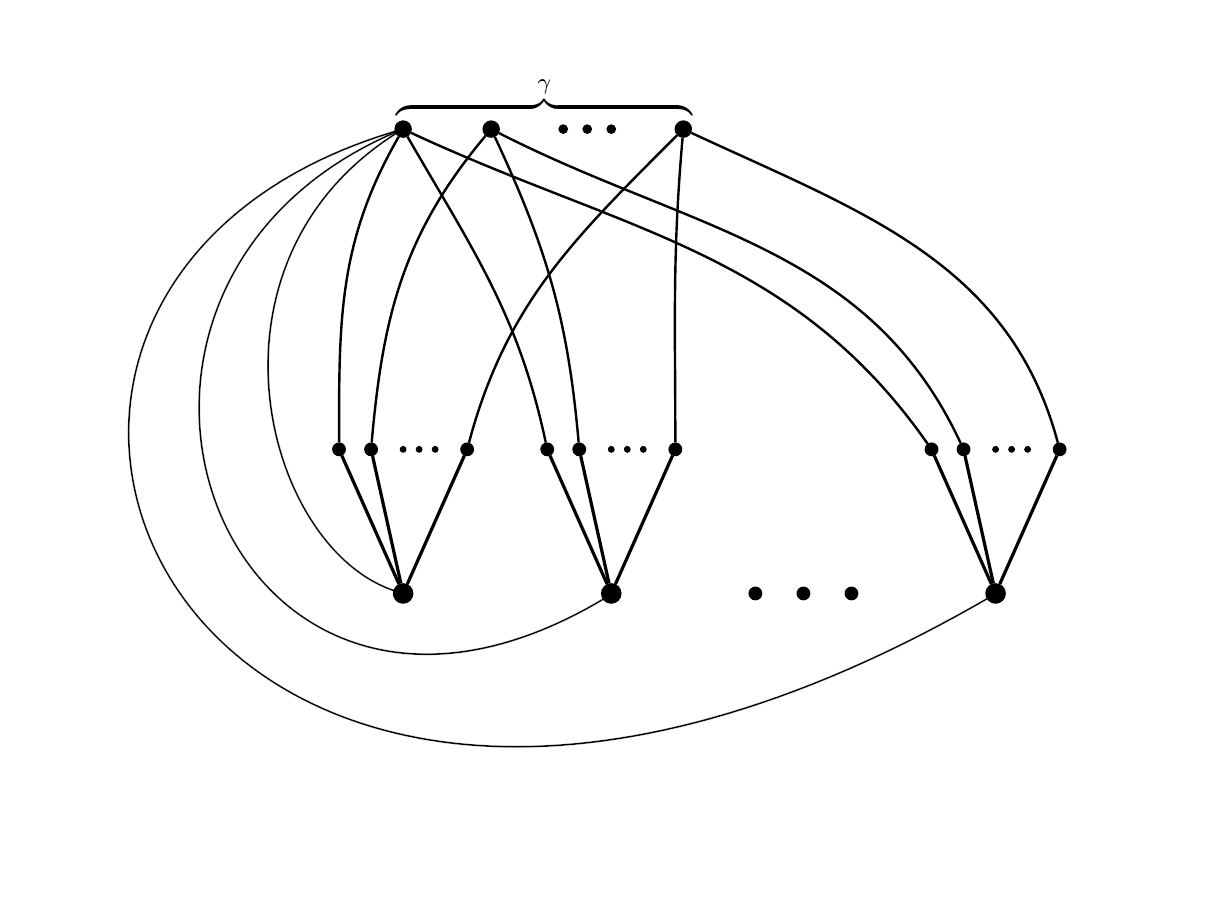
\includegraphics[scale=0.3]{ds1.png}

    \vspace{-3mm}
    \caption{ A $2$-degenerate graph, where for many $v\in V(G)$ the set $N(v)$ can only be dominated by at least $\gamma$ vertices different from $v$. }
  \end{figure}\label{fig:example}
\end{center}
\end{example}
